%% ------------- Portuguese version ------------
% \documentclass{sbrt}
% \usepackage[english,brazil]{babel}
% \usepackage[utf8]{inputenc}
% \newtheorem{theorem}{Teorema}
%% ------------------------------------
%% If writing in English, remove the lines above
%% and uncomment the lines below

%% ------------- English version ---------------
\documentclass[english]{sbrt}
\usepackage[utf8]{inputenc}
\usepackage{cite}
\usepackage{graphicx}
\usepackage{float}
\usepackage[top=2cm,left=2cm,right=3cm,bottom=3cm]{geometry}
\usepackage{titlesec}
\usepackage[center]{caption}
\newtheorem{theorem}{Theorem}
%% ---------------------------------------------

\titlespacing*{\section}
  {0pt}{18pt}{18pt}
  
\titlespacing*{\subsection}
  {0pt}{18pt}{18pt}

\begin{document}

% \graphicspath{{assets/}}

\title{Websocket delay analysis in browser-based multiplayer games}

\author{Tiago da Silva Guerreiro and Lucas Costa dos Prazeres
  \thanks{Special thanks to professor Eduardo Cerqueira, ITEC, UFPA, Belém-PA, e-mail: cerqueira@ufpa.br}
}

\maketitle

\baselineskip = 18pt


\begin{abstract}
  With the demand for low latency browser-based multiplayer games becoming higher as time passes, technologies like Websocket turn out to be essential in game development. In this paper, an analisys of the websocket traffic, more specifically its latency, is performed on a simple game. The results suggest that the number of players in the game can affect the game's latency by a significant amount.
\end{abstract}

\begin{keywords}

\end{keywords}

\section{\textbf{Introduction}}
Browser-based multiplayer games have been very popular in the recent years. The wide variety of devices supported and the seemingly unexistent installation process are some attractives that justify this exponential growth. However, multiplayer games in general require low latency and high throughput to deliver a satisfactory experience, since all the players' moves in the game have to be synced in both server and client as soon as possible. Further creation of the Websocket technology, in 2011, provided an excelent way to do so, by enabling bidirectional full-duplex communications over a single TCP connection, in contrast to long-pooling and other solutions that used HTTP.

This paper aims to analyze the Websocket traffic between both clients and server, using the previously made game in [reference].This article is organized as follows: Section II introduces the technologies used in this article, and Section III explains the changes made to the game in [reference]. Section IV explains how data used in the analisys was collected and plotted. The increase in latency presented, as more players connect to the server and move around, will be depicted in Section V.

\section{\textbf{Technical Background}}

This article's multiplayer game is designed in Javascript, using Node.js in backend, and Socket.io to establish Websocket communication.

\subsection{\textbf{Websocket}}
Websocket provides bidirectional full-duplex communication over a single TCP connection. Unlike HTTP, the websocket connection remains open until terminated by the server or client, which reduces the number of handshakes. Since the connection is already open, data transmission is faster.

The websocket technology is crucial to applications that require low latency, such as multiplayer browser-based games and streaming services.

\subsection{\textbf{Node.js}}
Node.js is a server environment that enables Javascript on the server side, without a browser. It uses an event-driven, asynchronous I/O, which makes Node.js capable of processing various requests simultaneously, and consequently, highly scalable.

Node.js provides a low cost, highly scalable environment for server-side applications. This technology is very useful on streaming web applications, real-time collaboration tools, online chats, microsservices and multiplayer games, since the server has to handle multiple requests from clients.

\subsection{\textbf{Socket.io}}
Socket.io is a Javascript library that enables Websocket capabilites in Javascript. With a few lines of code, an application can start listening to Websocket connections on the desired port. It is a very powerful tool to applications that depend on fast exchange of data, like multiplayer games.

\section{\textbf{Game changes}}

This version of the game has a few improvements, compared to what was presented in [reference]. Probably the most noticeable one is the addition of a scoreboard visible to all players in the match, which shows a relation of fruits collected per each player (represented as its websocket connection id). Moreover, an aesthetic improvement was made to the game so it could be closer to a regular game from the players's perspective, as shown in the fig. \ref{screen}.

\begin{figure}[H]
  \centering
  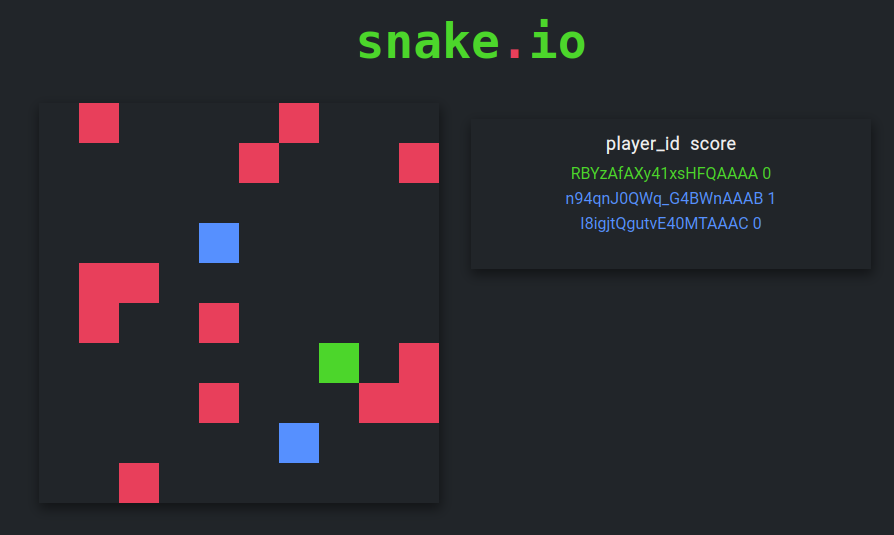
\includegraphics[width=10cm]{graphs/screen.png}
  \caption{New game layout (with 3 players connected)}
  \label{screen}
\end{figure}

Concerning to the game and network layer, the changes were respectively the points counting logic and
a few benchmarks inserted using the nodejs native function \textit{process.hrtime()}. The last one helped us understand how time related parameters of the network details in this project behave when
new players join the room, since it logs the websocket connection time and command-response delay on console when the browser loads the game.

\section{\textbf{Method}}

One essential network requirement of a multiplayer game is the ability to handle many connections (from many players) as gracefully as possible, while providing a good real-time game experience. This is why it is important to observe how time-related parameters behave on such applications, like delay or latency. This article manages to study how this temporal characteristic responds to linear variations on the number of active connections in a small experiment.

The experiment consists of a series of matches played with different numbers of clients and a single server hosting the game.
The server is a common laptop running \textit{Ubuntu Linux} with the backend game instance listening on localhost on port 3000. Since localhost applications usually are not acessible to hosts on different LANs, we used a port forwarding tool called \textit{ngrok}, which generated a tunnel using a USA located server to generate a public url to access the game server. Then, a few regular matches were played by clients located in different LANs - unlike the previous study [], in which the matches were played in a single LAN - while a native node.js function called \textit{process.hrtime()} collected temporal benchmarks in background showing the average time it took for the server to respond to every player move. The linear relation between both parameters was plotted using the Python library \textit{matplotlib} and are presented in the next section.

\section{\textbf{Results}}

The delay (or latency) is the time between an action and a system's reaction to it. In this particular context, it means the time it takes for the game server to notify all players when something changes on one of its clients, which could be a player moving, a fruit being removed or any other event triggered by an user interaction, from the moment an input is inserted on the keyboard. Since this response time depends on the whole network conditions from one host to another, it suffers variations even in similiar or identical game state scenarios, which brings the necessity of using statistical formulas like average or standard deviation to normalize the measured points. These techniques were applied to the experiment presented here and the results are depicted above.

Moreover, is important to point that this study faced a few challenges in terms of resources. For instance, all connections needed to be active and generate a sufficient data flow during the match, which means someone actually playing the game, in opposition to an idle client, and the number of available volunteers has limited how many samples could be collected on the experiment, making it difficult to analyze parameters other than the game latency. Nevertheless, it was possible to observe an increasing pattern on the latency measured with a linear variance on the number of players, as shown in Fig.\ref{latency}.

\begin{figure}[H]
  \centering
  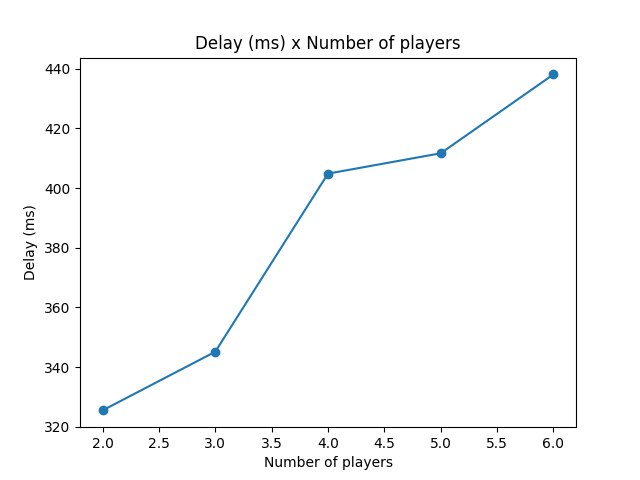
\includegraphics[width=10cm]{graphs/graph.png}
  \caption{Game latency with linear increasing on number of players}
  \label{latency}
\end{figure}

The results depict, as mentioned, a small increasing on the game latency, every time a new connection is established with the server. This was the expected behavior, after all each new client means a new packet being sent though the network, and due to the queue schema adopted by routers to handle priority of packets, in which the number of elements grows linearly, this also represents a similar raising pattern on latency. However, the fast data flow provided by the websocket protocol (as mentioned on section 2) attenuates the increasing on the response time, which could be higher if each packet was followed up by a handshake operation as it happens with regular HTTP transmissions.

\section{\textbf{Conclusion}}

The higher demand for real-time web applications for business purpouses, like fast collaboration tools and multiplayer games, was followed by an emergence of platforms and programming tools which support these needs. In this paper, the game latency is analyzed, as more players connect to the server and move around. The results suggest that the number of players in the game can affect the game's latency by a significant amount, due to the packets' priority in routing, but that's attenuated by the websocket protocol data flow. This factors really shows why websocket is essential in browser-based multiplayer games.

\cite{chen2011framework}

\bibliography{sbrt}
\bibliographystyle{IEEEtran}

\end{document}
